\documentclass[pdflatex,sn-mathphys-ay]{sn-jnl}

\usepackage{amsmath,amssymb,amsfonts}
\usepackage{graphicx}
\usepackage{booktabs}
\usepackage{array}
\usepackage{url}
\usepackage{amsthm}
\usepackage{float}
\usepackage{algorithm}
\usepackage{algorithmicx}
\usepackage{algpseudocode}
\usepackage{placeins}

\theoremstyle{thmstyleone}
\newtheorem{theorem}{Theorem}
\newtheorem{proposition}{Proposition}

\newcommand{\fhat}{\widehat{f}}
\newcommand{\fhatb}{\widehat{f}_b}
\newcommand{\stencil}{\mathcal{L}}
\newcommand{\orcidlink}[1]{\href{https://orcid.org/#1}{\raisebox{0.7ex}{\tiny ORCID}}}

\raggedbottom

\begin{document}

\title[Exact sparse traversal for grid-count density estimators]{Exact sparse traversal for local finite-stencil grid-count density estimators}

\author*[1]{\fnm{Aur{\'e}lien} \sur{Nicosia}\,\orcidlink{0000-0002-0974-9988}}
\email{aurelien.nicosia@mat.ulaval.ca}

\affil*[1]{\orgname{Universit{\'e} Laval}, \orgaddress{\city{Qu{\'e}bec}, \country{Canada}}}

\abstract{Grid-count density estimators replace sample-level interactions by operations on a regular lattice, but direct finite-stencil evaluation can waste work when most candidate grid cells are empty. This article studies exact sparse computation for local finite-stencil grid-count estimators, including histograms, averaged shifted histograms, linear blend frequency polygons, and generalized linear blend frequency polygons. We consider estimators of the form \(\fhatb(x)=(nV_b)^{-1}\sum_{\ell \in \stencil}\omega_\ell(x)\nu_{k(x)+\ell}\), where \(\stencil\) is a local stencil, \(\omega_\ell(x)\) are local weights, and \(\nu_k\) are grid counts. The proposed sparse-prefix traversal stores prefixes of occupied grid cells and prunes a branch only when no occupied cell has the current prefix. Thus the estimator, weights, bin widths, and boundary conventions are unchanged; only zero-count branches are skipped. For \(M\) query points, sparse traversal is favored when \(dG_{\mathrm{occ}}+M\bar p < M|\stencil|\), where \(G_{\mathrm{occ}}\) is the number of occupied cells and \(\bar p\) is the average number of prefix nodes tested per query point. Numerical checks confirm equality with direct evaluation at floating-point roundoff level. Benchmarks show speedups in sparse moderate-dimensional settings, while direct evaluation or convolutional methods remain preferable in regimes with small stencils, dense grids, or full-grid evaluation.}

\keywords{nonparametric density estimation, grid estimator, frequency polygon, averaged shifted histogram, sparse computation, computational statistics}

\maketitle

\section{Introduction}

Nonparametric density estimation is both a statistical smoothing problem and a computational representation problem. Ordinary kernel density estimators evaluate interactions between observations and query points. Grid-count estimators first aggregate observations into counts on a regular lattice, then evaluate densities from these counts. This aggregation is statistically interpretable and computationally useful because it separates count construction from subsequent density evaluation.

This article focuses on local finite-stencil grid-count estimators. After the grid counts have been constructed, each density value is obtained from a finite weighted sum of nearby grid counts. This class includes histograms, averaged shifted histograms, frequency polygons, and generalized linear blend frequency polygons \citep{Scott1985ASH,Scott1985FrequencyPolygon,Scott2015MDE}. Binned kernel estimators with compactly supported kernels, or Gaussian kernels explicitly truncated to a finite stencil, also fit this local grid-count form. Untruncated Gaussian binned KDEs are closely related, but they are better viewed as convolutional grid smoothers and may be more efficiently evaluated by separable convolution or FFT-based methods when the full grid is required \citep{Silverman1982FFT,Wand1994FastKDE,GramackiGramacki2017}.

The estimators considered here can be written as
\begin{equation}
\fhatb(x)
=
\frac{1}{nV_b}
\sum_{\ell \in \stencil}
\omega_\ell(x)\nu_{k(x)+\ell}.
\label{eq:general-estimator}
\end{equation}
Here \(X_1,\ldots,X_n\in\mathbb{R}^d\), \(b=(b_1,\ldots,b_d)\) is the vector of bin widths, \(V_b=\prod_{s=1}^d b_s\), \(k(x)\) is the grid cell associated with \(x\), \(\nu_k\) is the count in cell \(k\), \(\stencil\) is a local stencil, and \(\omega_\ell(x)\) is the weight attached to offset \(\ell\).

In this article, a local finite-stencil grid-count estimator means an estimator satisfying \eqref{eq:general-estimator} with a finite offset set \(\stencil\), weights \(\omega_\ell(x)\) determined by the query point and smoothing parameters, and counts \(\nu_k\) obtained from the sample on a regular grid. This is a computational class, not a claim about all linear density estimators. The method applies when the estimator can be evaluated by a finite local stencil of grid counts.

These estimators differ statistically but share the same computational issue. For the histogram, \(|\stencil|=1\), and evaluation requires a single count lookup. For the linear blend frequency polygon, abbreviated LBFP, the direct stencil size is \(2^d\). For averaged shifted histograms, abbreviated ASH, the stencil size is typically \(\prod_s(2m_s-1)\). For generalized linear blend frequency polygons, abbreviated GLBFP, a product-form stencil has size \(\prod_s 2m_s\). As \(|\stencil|\) grows with dimension or smoothing order, direct evaluation scans many candidate cells that may have zero counts.

Let
\[
K_{\mathrm{occ}}
=
\{k:\nu_k>0\}
\]
be the set of occupied cells, with \(G_{\mathrm{occ}}=|K_{\mathrm{occ}}|\). If a candidate cell \(k(x)+\ell\) is not in \(K_{\mathrm{occ}}\), its contribution to \eqref{eq:general-estimator} is exactly zero. Sparse count maps reduce memory and make individual lookups cheap, but they do not by themselves remove the loop over all offsets in \(\stencil\). The computational question is whether impossible offsets can be avoided without changing the estimator.

We formulate an exact sparse-prefix traversal for this purpose. The method stores prefixes of occupied cell coordinates under a chosen dimension ordering and traverses the local stencil recursively. Whenever the current coordinate prefix is incompatible with all occupied cells, the entire branch is pruned. At a leaf, the algorithm adds the corresponding exact weighted contribution. The traversal changes the computation but not the estimator: it does not approximate small weights, modify bin widths, change boundary conventions, or replace the grid. It removes only terms whose grid count is exactly zero.

The benefit of sparse traversal is not guaranteed. Let \(x^{(1)},\ldots,x^{(M)}\) be the points at which the estimator is evaluated. The direct cost per query point is \(|\stencil|\). If \(p_i\) denotes the number of prefix nodes tested for the \(i\)-th query point, then the sparse-prefix cost is approximately
\begin{equation}
T_{\mathrm{sparse}}
\approx
dG_{\mathrm{occ}}+\sum_{i=1}^M p_i,
\label{eq:sparse-cost}
\end{equation}
where \(dG_{\mathrm{occ}}\) is the cost of constructing the prefix index. Direct evaluation costs
\begin{equation}
T_{\mathrm{direct}}
\approx
M|\stencil|.
\label{eq:direct-cost}
\end{equation}
Sparse traversal is therefore expected to be useful when
\begin{equation}
dG_{\mathrm{occ}}+M\bar p
<
M|\stencil|,
\label{eq:mode-criterion}
\end{equation}
where \(\bar p=M^{-1}\sum_{i=1}^M p_i\). When the density is evaluated at the original observations, as in leave-one-out scores or observation-level diagnostics, \(M=n\). This observation-only regime is particularly relevant when the estimator must be evaluated at all sample points but not necessarily on the full grid. This inequality is the main computational criterion of the paper. It shows that dimension is only one part of the computational regime: sparse traversal also depends on grid occupancy, local sparsity, prefix ordering, and the number of query points.

The sparse-prefix traversal should be viewed as a specialization of standard sparse-computation ideas to a specific statistical task. Sparse maps, tries, coordinate fibers, and compressed sparse representations are established tools \citep{Fredkin1960Trie,BaderKolda2007SparseTensor,KoldaBader2009TensorReview}. The paper does not claim a new general-purpose sparse data structure. Its contribution is the estimator-specific formulation, exact pruning rule, exactness argument, and cost criterion for choosing between direct and sparse evaluation.

The contributions of the article are as follows: (i) a common finite-stencil grid-count formulation for histograms, ASH, LBFP, and GLBFP; (ii) an exact sparse-prefix traversal that prunes only stencil branches that cannot contain occupied cells; (iii) an exactness result showing that sparse traversal returns the same estimator as direct stencil evaluation, up to floating-point summation order; and (iv) a cost criterion and pilot-based mode selector comparing \(dG_{\mathrm{occ}}+M\bar p\) with \(M|\stencil|\). The novelty lies in this combination for local grid-count density estimators, not in the generic existence of sparse data structures. This is therefore a computational contribution: it provides an exact evaluation strategy and a mode-selection criterion for existing finite-stencil grid-count estimators, rather than proposing a new density estimator.

The rest of the article is organized as follows. Section~\ref{sec:grid-estimators} introduces the common grid-count notation and presents the estimator family. Section~\ref{sec:sparse-traversal} describes direct and sparse-prefix evaluation. Section~\ref{sec:cost} develops the cost criterion and automatic mode selector. Section~\ref{sec:experiments} reports numerical validation checks and scaling benchmark results. Section~\ref{sec:discussion} discusses estimator-specific regimes, limitations, and future work.

\section{Local finite-stencil grid-count estimators}
\label{sec:grid-estimators}

\subsection{Common grid notation}

Let \(X_1,\ldots,X_n\in\mathbb{R}^d\). A regular grid is specified by an origin \(a_0\in\mathbb{R}^d\) and bin widths \(b=(b_1,\ldots,b_d)\). For \(x\in\mathbb{R}^d\), define the cell index
\[
k_s(x)
=
\left\lfloor
\frac{x_s-a_{0s}}{b_s}
\right\rfloor,
\qquad s=1,\ldots,d.
\]
Let \(k(x)=(k_1(x),\ldots,k_d(x))\), and let \(\nu_k\) be the number of observations assigned to cell \(k\). The bin volume is \(V_b=\prod_s b_s\).
Unless otherwise stated, grid cells are the half-open rectangles
\[
\prod_{s=1}^d
\left[a_{0s}+k_sb_s,\ a_{0s}+(k_s+1)b_s\right),
\]
so points on grid boundaries are assigned by the floor convention above. The same boundary convention is used throughout the paper.

All estimators considered here are finite local weighted sums of grid counts. They differ by the stencil \(\stencil\) and by the weight function \(\omega_\ell(x)\). Table~\ref{tab:estimators} summarizes the relevant stencil sizes.

\begin{table}[t]
\centering
\caption{Local stencil size for the finite-stencil grid-count estimators considered in this article.}
\label{tab:estimators}
\begin{tabular}{lll}
\toprule
Estimator & Stencil \(\stencil\) & Nominal size \(S=|\stencil|\) \\
\midrule
Histogram & \(\{0\}\) & \(1\) \\
LBFP & \(\{0,1\}^d\) & \(2^d\) \\
ASH & \(\prod_s \{1-m_s,\ldots,m_s-1\}\) & \(\prod_s(2m_s-1)\) \\
GLBFP & \(\prod_s \{1-m_s,\ldots,m_s\}\) & \(\prod_s 2m_s\) \\
\bottomrule
\end{tabular}
\end{table}

\subsection{Histogram}

The histogram estimator is
\[
\fhatb^{\mathrm{hist}}(x)
=
\frac{\nu_{k(x)}}{nV_b}.
\]
Its stencil size is one. Sparse-prefix traversal is not useful for histograms because direct evaluation is already a single lookup.

\subsection{Linear blend frequency polygon}

For LBFP, let
\[
u_s(x)
=
\frac{x_s-a_{0s}-k_s(x)b_s}{b_s}
\in [0,1)
\]
be the local coordinate in dimension \(s\), with boundary cases handled by the half-open cell convention. For \(j\in\{0,1\}^d\), define
\[
c_j(x)
=
\prod_{s=1}^d
u_s(x)^{j_s}\{1-u_s(x)\}^{1-j_s}.
\]
These weights satisfy \(\sum_{j\in\{0,1\}^d}c_j(x)=1\), so the LBFP is a convex local blend of neighboring histogram counts.
Then
\begin{equation}
\fhatb^{\mathrm{LBFP}}(x)
=
\frac{1}{nV_b}
\sum_{j\in\{0,1\}^d}
c_j(x)\nu_{k(x)+j}.
\label{eq:lbfp}
\end{equation}
Frequency polygons have a long history in density estimation \citep{Scott1985FrequencyPolygon,Scott2015MDE}, and recent work studies multivariate versions in dependent random-field settings \citep{CarbonDuchesne2024}. Computationally, \eqref{eq:lbfp} has stencil size \(2^d\), which makes it the simplest nontrivial case for sparse traversal.

\subsection{Averaged shifted histograms}

ASH estimators average shifted histograms, often using triangular weights \citep{Scott1985ASH}. With refinement parameters \(m=(m_1,\ldots,m_d)\), a product-form ASH stencil can be written as
\[
\fhatb^{\mathrm{ASH}}(x)
=
\frac{1}{nV_b}
\sum_{\ell_1=1-m_1}^{m_1-1}
\cdots
\sum_{\ell_d=1-m_d}^{m_d-1}
\left\{
\prod_{s=1}^d
\left(1-\frac{|\ell_s|}{m_s}\right)
\right\}
\nu_{k(x)+\ell}.
\]
This is the computational finite-stencil form of the averaged shifted histogram under the refinement parameters \(m_s\). The ASH stencil is
\(\stencil=\prod_s\{1-m_s,\ldots,m_s-1\}\), with size \(\prod_s(2m_s-1)\). Sparse traversal can be applied, but convolution or FFT-based methods may be preferable when the full grid is required and \(G\) is moderate \citep{Silverman1982FFT,GramackiGramacki2017}.

\subsection{Generalized linear blend frequency polygons}

GLBFP estimators combine refined-grid averaging and linear blending. In the product-form representation used here, the stencil can be written as
\[
\fhatb^{\mathrm{GLBFP}}(x)
=
\frac{1}{nV_b}
\sum_{\ell_1=1-m_1}^{m_1}
\cdots
\sum_{\ell_d=1-m_d}^{m_d}
\left\{\prod_{s=1}^d W_s(\ell_s;u_s)\right\}
\nu_{k(x)+\ell},
\]
where \(u_s=u_s(x)\), \((t)_+=\max(t,0)\), and
\[
W_s(\ell;u_s)
=
(1-u_s)\left(1-\frac{|\ell|}{m_s}\right)_+
+
u_s\left(1-\frac{|\ell-1|}{m_s}\right)_+.
\]
This weight has a direct ASH plus linear blend interpretation. In one dimension, the left ASH value contributes a triangular weight centered at offset \(\ell\), multiplied by \(1-u_s\). The right ASH value contributes a triangular weight centered at offset \(\ell-1\), multiplied by \(u_s\). Adding these two contributions gives \(W_s(\ell;u_s)\), and the \(d\)-dimensional product structure follows from the tensor-product construction.

The product-form expression above is algebraically equivalent to the ASH plus linear blend definition of the GLBFP under the grid convention used here. It is written in this form because sparse-prefix traversal operates directly on finite stencil offsets and their weights. When \(m_s=1\), the only nonzero one-dimensional weights correspond to \(\ell_s\in\{0,1\}\), with weights \(1-u_s\) and \(u_s\), recovering the LBFP stencil. For \(m_s>1\), the nominal stencil size is \(\prod_s 2m_s\), so the potential benefit of sparse traversal can be substantial in sparse grids.

These examples reduce several density estimators to the same computational task: evaluating a finite weighted stencil of grid counts. The next section describes direct evaluation and the sparse-prefix alternative for this common task.

\section{Direct and sparse-prefix evaluation}
\label{sec:sparse-traversal}

The finite-stencil representation in Section~\ref{sec:grid-estimators} separates the statistical definition of an estimator from the computational method used to evaluate it. This section compares direct stencil enumeration with exact sparse-prefix traversal.

\subsection{Direct sparse-count evaluation}

A direct implementation first constructs a sparse count map for the occupied cells and then evaluates \eqref{eq:general-estimator} by looping over every \(\ell\in\stencil\). Each candidate count is obtained by a hash lookup or an array lookup. This representation reduces memory from \(O(G)\) to \(O(G_{\mathrm{occ}})\), but the evaluation cost remains \(O(|\stencil|)\) per query point. Algorithm~\ref{alg:direct-stencil} gives the direct stencil evaluation for a fixed query point.

\begin{algorithm}[H]
\caption{Direct stencil evaluation}
\label{alg:direct-stencil}
\begin{algorithmic}[1]
\Require Query point \(x\), sparse count map \(\nu\), stencil \(\stencil\), weights \(\omega_\ell(x)\), sample size \(n\), bin volume \(V_b\)
\Ensure \(\fhatb(x)\)
\State \(k \gets k(x)\)
\State \(\mathrm{total} \gets 0\)
\ForAll{\(\ell\in\stencil\)}
  \State \(c \gets k+\ell\)
  \State \(m \gets \nu_c\) if \(c\) is present in the sparse count map, and \(m \gets 0\) otherwise
  \State \(\mathrm{total} \gets \mathrm{total}+\omega_\ell(x)m\)
\EndFor
\State \Return \(\mathrm{total}/(nV_b)\)
\end{algorithmic}
\end{algorithm}

\subsection{Prefix index}

Let \(\pi\) be a permutation of \(\{1,\ldots,d\}\). For an occupied cell \(k\in K_{\mathrm{occ}}\), define its ordered prefix of depth \(r\) as
\[
\operatorname{pref}_r(k)
=
(k_{\pi_1},\ldots,k_{\pi_r}).
\]
The prefix index stores
\[
P_r
=
\{\operatorname{pref}_r(k):k\in K_{\mathrm{occ}}\},
\qquad r=1,\ldots,d.
\]
The implementation may use hash sets, tries, compressed sparse tensors, or sorted coordinate fibers. The current reference implementation uses hash sets for clarity.

\subsection{Relation to generic sparse traversal}

A prefix index can be implemented in many ways: hash sets of prefixes, a trie, sorted coordinate fibers, compressed sparse tensor structures, or other sparse multidimensional indexes. The algorithms in this article use prefix sets for clarity, not because hash sets are necessarily optimal. The exactness statement is data-structure independent: any implementation is exact if it prunes a branch only when no occupied cell has the current ordered prefix. Computational constants may vary substantially across implementations, but the cost comparison captures the leading trade-off between direct stencil enumeration and sparse branch pruning.

\subsection{Traversal}

For a query point \(x\), the local stencil gives a finite set of candidate coordinates in each dimension. LBFP has two candidates per dimension, \(k_s(x)\) and \(k_s(x)+1\). ASH and GLBFP have larger candidate sets determined by \(m_s\). The sparse-prefix algorithm traverses these candidates in the order \(\pi\). Whenever the current ordered prefix is not in \(P_r\), the branch is pruned. Prefixes are tested in the ordering \(\pi\), while the final leaf is converted back to the original coordinate order before querying the count map.

Algorithm~\ref{alg:sparse-prefix} formalizes the traversal for the product-form stencils used here. Let \(C_s(x)\) denote the candidate coordinates in dimension \(s\), with one-dimensional weight \(a_s(c_s;x)\). A candidate cell \(c=(c_1,\ldots,c_d)\) has weight
\[
a(c;x)=\prod_{s=1}^d a_s(c_s;x).
\]
In the recursion, \(\rho\) denotes the current ordered prefix and \(w\) denotes the accumulated product weight. At a leaf, an ordered vector \(\rho'=(q_1,\ldots,q_d)\) is converted to the original coordinate order by setting \(c_{\pi_j}=q_j\) for \(j=1,\ldots,d\). The count map is then queried with the full cell \(c=(c_1,\ldots,c_d)\). For a non-product stencil, the recursion can instead carry a lookup of the corresponding \(\omega_\ell(x)\) at the leaf.

\begin{algorithm}[H]
\caption{Sparse-prefix traversal}
\label{alg:sparse-prefix}
\begin{algorithmic}[1]
\Require Query point \(x\), prefix sets \(P_1,\ldots,P_d\), occupied count map \(\nu\), coordinate candidate sets \(C_s(x)\), coordinate weights \(a_s(\cdot;x)\), sample size \(n\), bin volume \(V_b\), ordering \(\pi\)
\Ensure \(\fhatb(x)\)
\State \(\mathrm{total} \gets 0\)
\Statex \(\rho\) is an ordered prefix; \(w\) is the accumulated product weight.
\Procedure{Visit}{$r,\rho,w$}
  \State \(s \gets \pi_r\)
  \ForAll{\(c_s\in C_s(x)\)}
    \State \(\rho' \gets (\rho,c_s)\)
    \State \(w' \gets w\,a_s(c_s;x)\)
    \If{\(\rho' \notin P_r\)}
      \State \textbf{continue} \Comment{no occupied cell has this prefix}
    \EndIf
    \If{\(r=d\)}
      \State \(c \gets \operatorname{unpermute}_{\pi}(\rho')\)
      \State \(m \gets \nu_c\) if \(c\) is present in the occupied count map, and \(m \gets 0\) otherwise
      \State \(\mathrm{total} \gets \mathrm{total}+w'm\)
    \Else
      \State \Call{Visit}{$r+1,\rho',w'$}
    \EndIf
  \EndFor
\EndProcedure
\State \Call{Visit}{$1,\emptyset,1$}
\State \Return \(\mathrm{total}/(nV_b)\)
\end{algorithmic}
\end{algorithm}

\subsection{Exactness}

Theorem~\ref{thm:sparse-exactness} states the exactness guarantee for sparse-prefix traversal.

\begin{theorem}[Exactness of sparse-prefix traversal]
\label{thm:sparse-exactness}
For any fixed query point \(x\), finite stencil \(\stencil\), local weights \(\omega_\ell(x)\), and sparse count map \(\nu\), let the occupied cell set be
\[
K_{\mathrm{occ}}
=
\{k:\nu_k>0\}.
\]
The displayed Algorithm~\ref{alg:sparse-prefix} corresponds to product-form stencils. For a general finite stencil, the same traversal is used with the corresponding local weight \(\omega_\ell(x)\) evaluated at the leaf. In either case, sparse-prefix traversal returns the same value \(\fhatb(x)\) as direct stencil evaluation, up to floating-point summation order.
\end{theorem}

\begin{proof}
The direct stencil sum can be decomposed into occupied and unoccupied candidate cells:
\[
\sum_{\ell\in\stencil}
\omega_\ell(x)\nu_{k(x)+\ell}
=
\sum_{\ell:k(x)+\ell\in K_{\mathrm{occ}}}
\omega_\ell(x)\nu_{k(x)+\ell}
+
\sum_{\ell:k(x)+\ell\notin K_{\mathrm{occ}}}
\omega_\ell(x)\nu_{k(x)+\ell}.
\]
The second sum is exactly zero by definition of \(K_{\mathrm{occ}}\). A prefix branch is pruned only if no occupied cell has the current ordered prefix. Therefore no occupied candidate cell can be removed by the traversal. In the product-form case, the leaf weight accumulated by Algorithm~\ref{alg:sparse-prefix} is \(a(c;x)\). In the general finite-stencil case, the corresponding implementation evaluates \(\omega_\ell(x)\) at the leaf. Thus sparse-prefix traversal sums exactly the same nonzero terms as Algorithm~\ref{alg:direct-stencil}, with only the order of floating-point additions possibly changed.
\end{proof}

\section{Cost model and mode selection}
\label{sec:cost}

\begin{proposition}[Cost criterion for sparse-prefix evaluation]
\label{prop:cost-criterion}
Let \(S=|\stencil|\), and suppose the estimator is evaluated at \(M\) query points. Direct evaluation has nominal cost
\[
T_{\mathrm{direct}}=O(MS).
\]
Sparse-prefix evaluation has index construction cost \(O(dG_{\mathrm{occ}})\) and traversal cost proportional to the number of prefix nodes tested:
\[
T_{\mathrm{sparse}}
=
O(dG_{\mathrm{occ}})
+
O\left(\sum_{i=1}^M p_i\right).
\]
With
\[
\bar p
=
\frac{1}{M}\sum_{i=1}^M p_i,
\]
sparse traversal is attractive when
\[
dG_{\mathrm{occ}}+M\bar p
<
MS.
\]
\end{proposition}

\begin{proof}
Algorithm~\ref{alg:direct-stencil} tests all \(S=|\stencil|\) stencil offsets for each of the \(M\) query points, giving \(O(MS)\) nominal work. Sparse-prefix traversal first constructs prefix sets for occupied cells. Storing prefixes over \(d\) dimensions for \(G_{\mathrm{occ}}\) occupied cells costs \(O(dG_{\mathrm{occ}})\). During evaluation, the \(i\)-th query point tests \(p_i\) prefix nodes, so the traversal work is proportional to \(\sum_{i=1}^M p_i=M\bar p\). Comparing the two leading work counts gives the stated criterion.
\end{proof}

Proposition~\ref{prop:cost-criterion} is useful because sparse storage alone does not determine the best evaluation strategy. A sparse count map reduces memory and lookup cost, but direct evaluation still scans all \(S=|\stencil|\) offsets. Conversely, sparse-prefix traversal incurs an index-construction cost and recursive traversal overhead. The criterion \(dG_{\mathrm{occ}}+M\bar p<M|\stencil|\) identifies the regime in which pruning enough zero-count branches compensates for this overhead, making the computational mode practically selectable rather than purely heuristic.

For histograms, \(S=1\), so direct evaluation should be used. For LBFP, \(S=2^d\), so sparse-prefix traversal becomes attractive when local occupancy is sparse enough that \(\bar p\ll 2^d\). For ASH and GLBFP, \(S\) also depends on the smoothing parameters \(m_s\). These estimators may benefit from sparse traversal for pointwise evaluation in sparse high-dimensional grids, but convolutional methods may be superior when the whole grid is needed and \(G\) is manageable \citep{Silverman1982FFT,Wand1994FastKDE,GramackiGramacki2017}.

An automatic mode selector can be based on a short pilot run. First build the occupied-cell representation and compute \(G_{\mathrm{occ}}\). Then estimate \(\bar p\) on a subset of evaluation points. Select sparse traversal if
\[
dG_{\mathrm{occ}}+M\widehat{\bar p}
<
\tau M|\stencil|,
\]
where \(\tau<1\) is a safety factor, for example \(\tau=0.8\). Here \(M=n\) for observation-only evaluation. Otherwise select direct evaluation. This rule avoids a dimension-only threshold and adapts to the observed grid occupancy and evaluation task.

\section{Numerical validation and scaling benchmarks}
\label{sec:experiments}

The numerical study first verifies exactness at the implementation level, then examines when sparse-prefix traversal reduces computational cost. This ordering is important because timing comparisons are meaningful only after confirming equality with direct stencil evaluation.

\subsection{Correctness checks}

The first validation step checks numerical equality against direct stencil evaluation in tractable settings. These checks verify the exactness statement in Theorem~\ref{thm:sparse-exactness} at the implementation level. Correctness checks were run for \(n\in\{100,500\}\), \(d\in\{2,3,5,8\}\), two bin settings, and two synthetic scenarios. The reference R and C++ implementations both agreed with direct LBFP evaluation. Across 64 rows, the maximum absolute density error was \(8.88\times 10^{-16}\). Additional estimator-family checks for ASH, LBFP, and GLBFP also agreed with direct stencil evaluation, with maximum absolute errors below \(6\times 10^{-17}\). The observed discrepancies are at floating-point roundoff level, consistent with the fact that sparse traversal changes only the summation path.

\subsection{Estimator-family coverage}

Because the proposed traversal is formulated for local finite-stencil grid-count estimators, the numerical study distinguishes estimator coverage from optimized runtime. The first question is whether the same exact sparse-prefix idea applies beyond LBFP. The second is how much performance can be obtained by a compiled implementation. To address the first question, a reference implementation was evaluated for histogram, ASH with \(m=2\), LBFP, and GLBFP with \(m=2\), using \(n\in\{250,500,1000,2000\}\), \(d=2,\ldots,6\), and one replication. Histograms are reported as direct lookup only because their stencil size is one. Very large direct-stencil GLBFP configurations were omitted to keep the comparison within the intended computational scope.

Table~\ref{tab:family-benchmark} summarizes the estimator-family benchmark. This experiment is intended to assess estimator-family coverage rather than optimized runtime. It verifies that the same exact pruning mechanism applies beyond LBFP, while the compiled LBFP study below isolates algorithmic speedup in an optimized backend. The results also show that the benefit becomes clearer as the nominal stencil grows.

\begin{table}[t]
\centering
\caption{Estimator-family benchmark from the R implementation. Histograms are omitted because they use direct lookup only.}
\label{tab:family-benchmark}
\begin{tabular}{lrrrr}
\toprule
Estimator & tested \(d\) & max speedup & \(d_{\max}\) & max error \\
\midrule
ASH   & 2--6 & 10.50 & 6 & \(0.00\) \\
LBFP  & 2--6 & 2.47 & 6 & \(4.16\times 10^{-17}\) \\
GLBFP & 2--6 & 22.00 & 6 & \(5.55\times 10^{-17}\) \\
\bottomrule
\end{tabular}
\end{table}

Figures~\ref{fig:family-speedup} and~\ref{fig:family-speedup-lines} give the corresponding visual summaries. They also make clear why histograms should not be handled by sparse-prefix traversal: direct lookup is already the full estimator evaluation.

\begin{figure}[t]
\centering
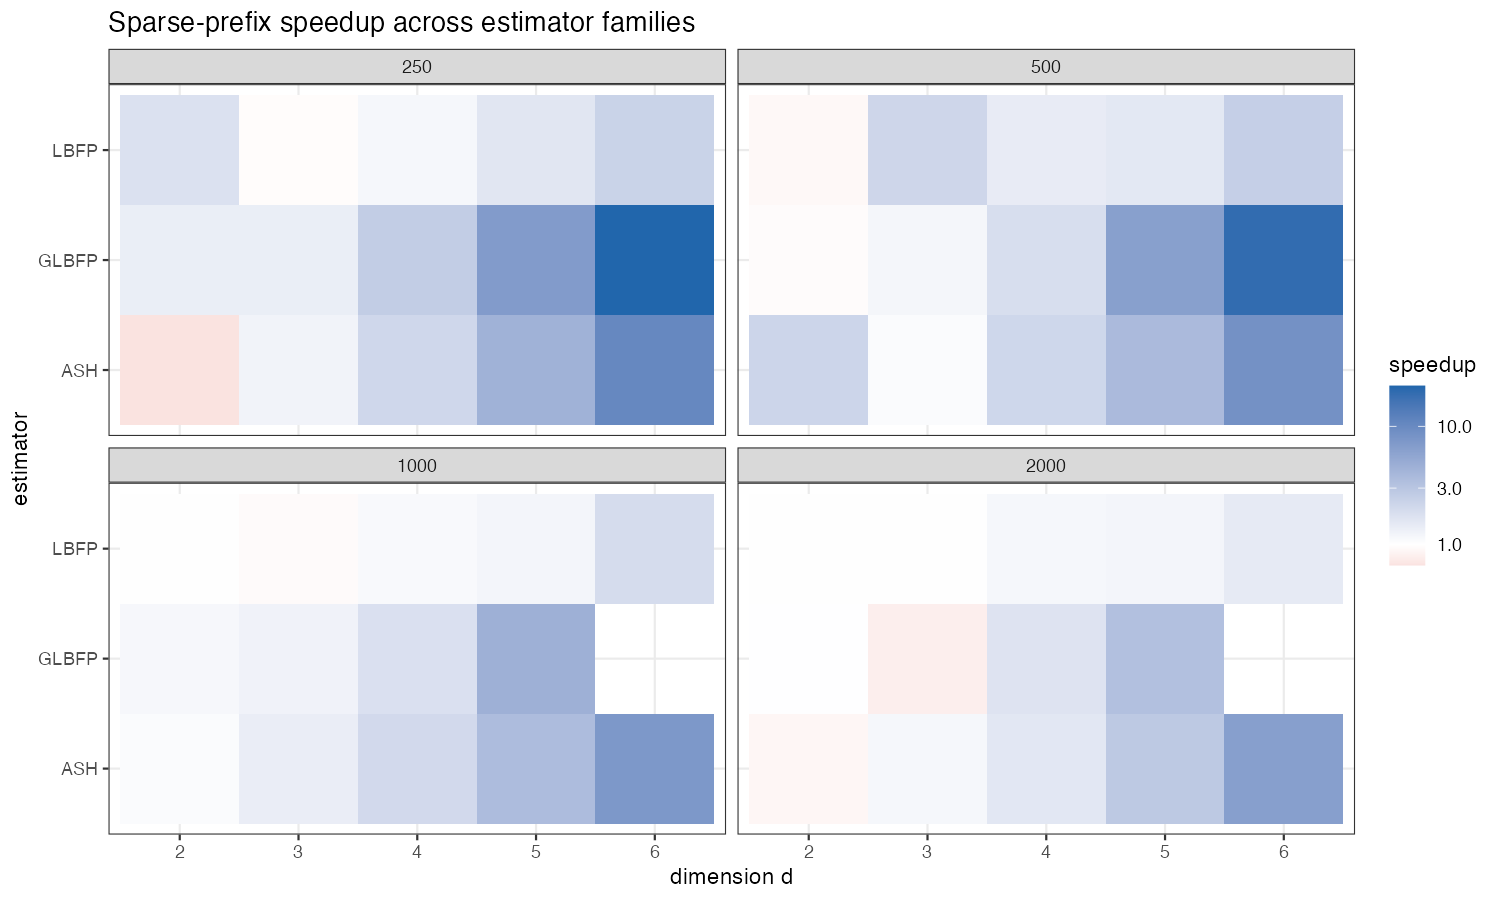
\includegraphics[width=0.95\textwidth]{../code/figures/estimator_family_speedup_heatmap.png}
\caption{Sparse-prefix speedup relative to direct R stencil evaluation for ASH, LBFP, and GLBFP. Values below one indicate sparse-prefix overhead.}
\label{fig:family-speedup}
\end{figure}

\begin{figure}[t]
\centering
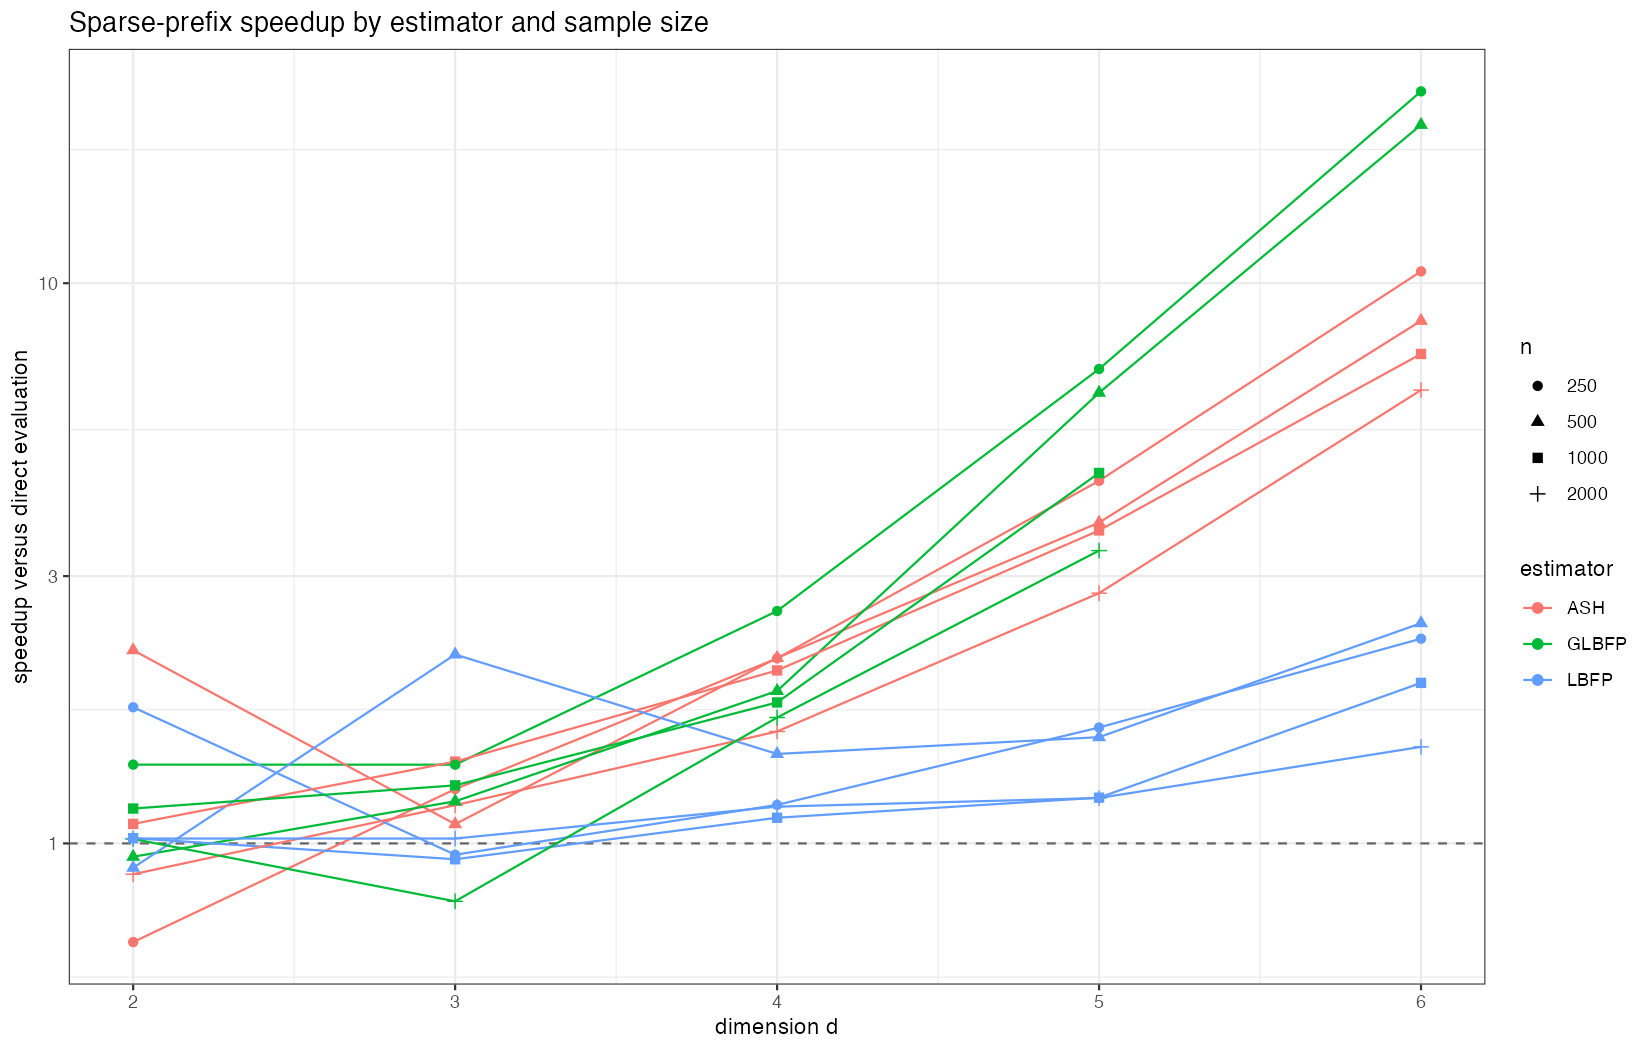
\includegraphics[width=0.95\textwidth]{../code/figures/estimator_family_speedup_by_dimension.png}
\caption{Sparse-prefix speedup relative to direct R stencil evaluation as a function of dimension. All estimator families and tested sample sizes are shown in a single panel.}
\label{fig:family-speedup-lines}
\end{figure}

\subsection{Scaling design}

The second timing study focuses on LBFP. It compares two compiled backends: direct C++ stencil evaluation and sparse-prefix C++ traversal. This comparison isolates algorithmic gain from programming-language effects. The scaling grid uses sample sizes from 500 to 10000, dimensions \(d=2,\ldots,12\), two outer replications, and ten inner timing repetitions for each backend. All timing records are retained only after checking equality between direct and sparse-prefix values.

This experiment is a controlled scaling study designed to isolate the transition between direct and sparse-prefix evaluation as \(d\) and \(n\) vary. It uses a fixed synthetic data-generating mechanism so that changes in runtime can be attributed primarily to dimension, sample size, occupancy, and prefix traversal behavior.

\subsection{Transition with dimension and sample size}

Table~\ref{tab:scaling-transition} summarizes the observed transition. The column \(d_{\mathrm{first}}\) is the first dimension, in the grid \(2,\ldots,12\), for which the median sparse-prefix time is smaller than the median direct C++ time. The prefix ratio is the median number of tested prefix nodes divided by \(2^d\), minimized over the tested dimensions for each \(n\).

\begin{table}[!htbp]
\centering
\caption{LBFP scaling diagnostics from the \(n\)-by-\(d\) benchmark. Speedups are measured against the direct C++ backend.}
\label{tab:scaling-transition}
\begin{tabular}{rrrrrr}
\toprule
\(n\) & \(d_{\mathrm{first}}\) & max speedup & \(d\) at max & min prefix ratio & max error \\
\midrule
500   & 6 & 46.50 & 12 & 0.036 & \(1.39\times 10^{-17}\) \\
1000  & 7 & 33.42 & 12 & 0.044 & \(1.39\times 10^{-17}\) \\
2000  & 5 & 28.79 & 12 & 0.057 & \(3.47\times 10^{-17}\) \\
5000  & 5 & 55.87 & 12 & 0.078 & \(1.73\times 10^{-17}\) \\
10000 & 6 & 36.07 & 12 & 0.097 & \(2.08\times 10^{-17}\) \\
\bottomrule
\end{tabular}
\end{table}

\FloatBarrier

In low dimensions, the direct stencil has only \(4\), \(8\), or \(16\) vertices, so sparse-prefix traversal generally pays more overhead than it saves. The observed crossover occurs between \(d=5\) and \(d=7\). For \(d\geq 8\), all tested sample sizes show a speedup above \(2.8\), and the prefix ratio continues to decrease as \(d\) increases. The improvement is therefore mainly a function of the effective stencil sparsity induced by dimension and occupancy, not of \(n\) alone.

Figures~\ref{fig:scaling-heatmap}--\ref{fig:scaling-prefix} visualize the same transition from three complementary perspectives: speedup over the \(n\)-by-\(d\) grid, speedup as a function of dimension, and the corresponding prefix-node ratio.

\begin{figure}[!htbp]
\centering
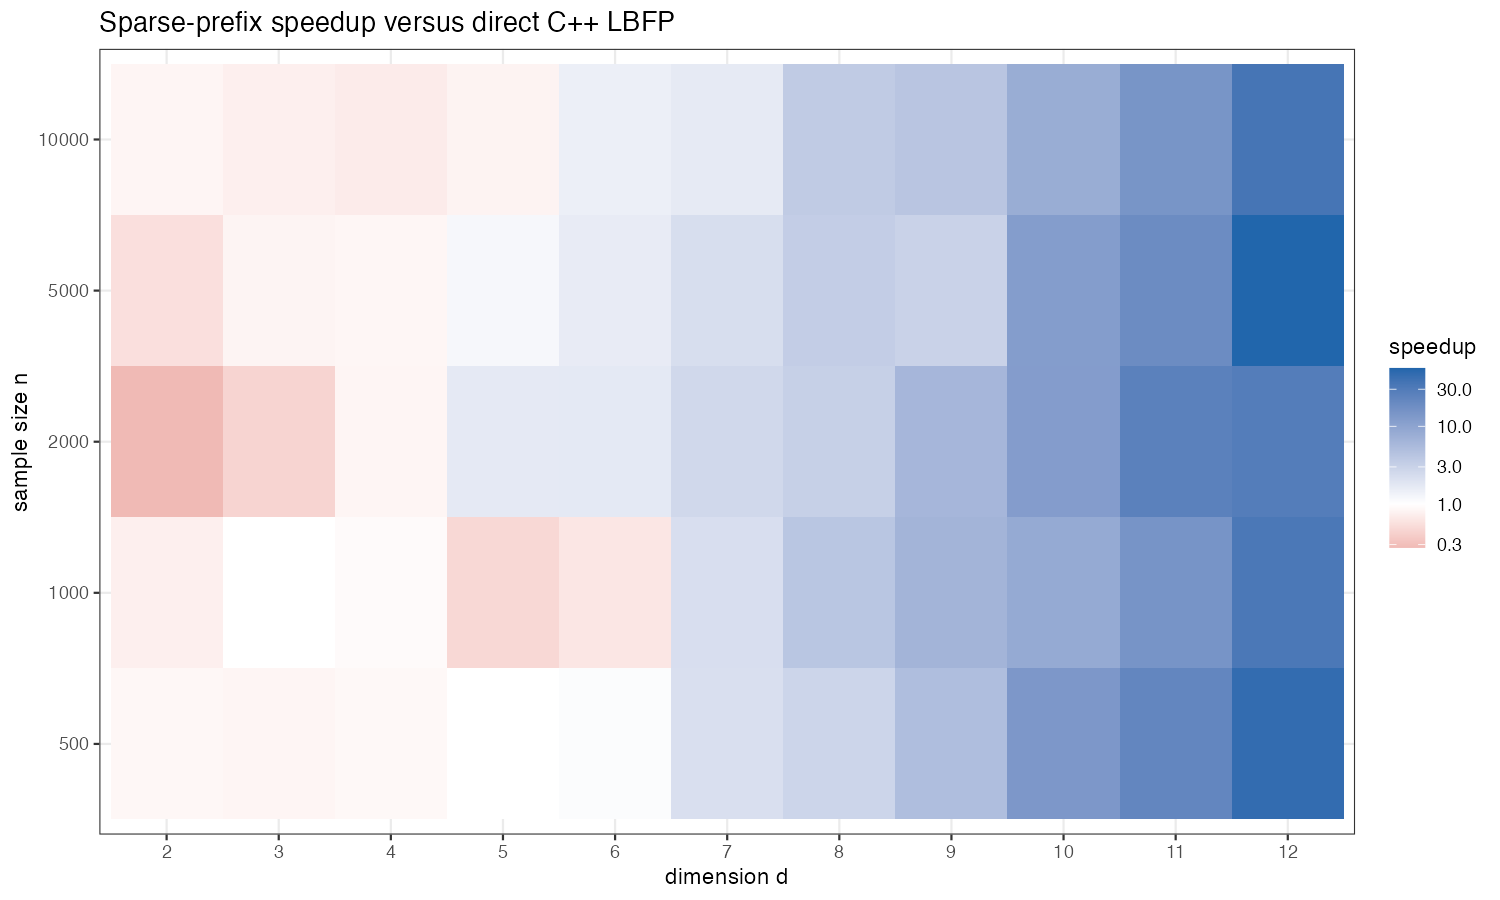
\includegraphics[width=0.95\textwidth]{../code/figures/scaling_speedup_heatmap.png}
\caption{Median sparse-prefix speedup relative to direct C++ LBFP evaluation across dimension and sample size.}
\label{fig:scaling-heatmap}
\end{figure}

\begin{figure}[!htbp]
\centering
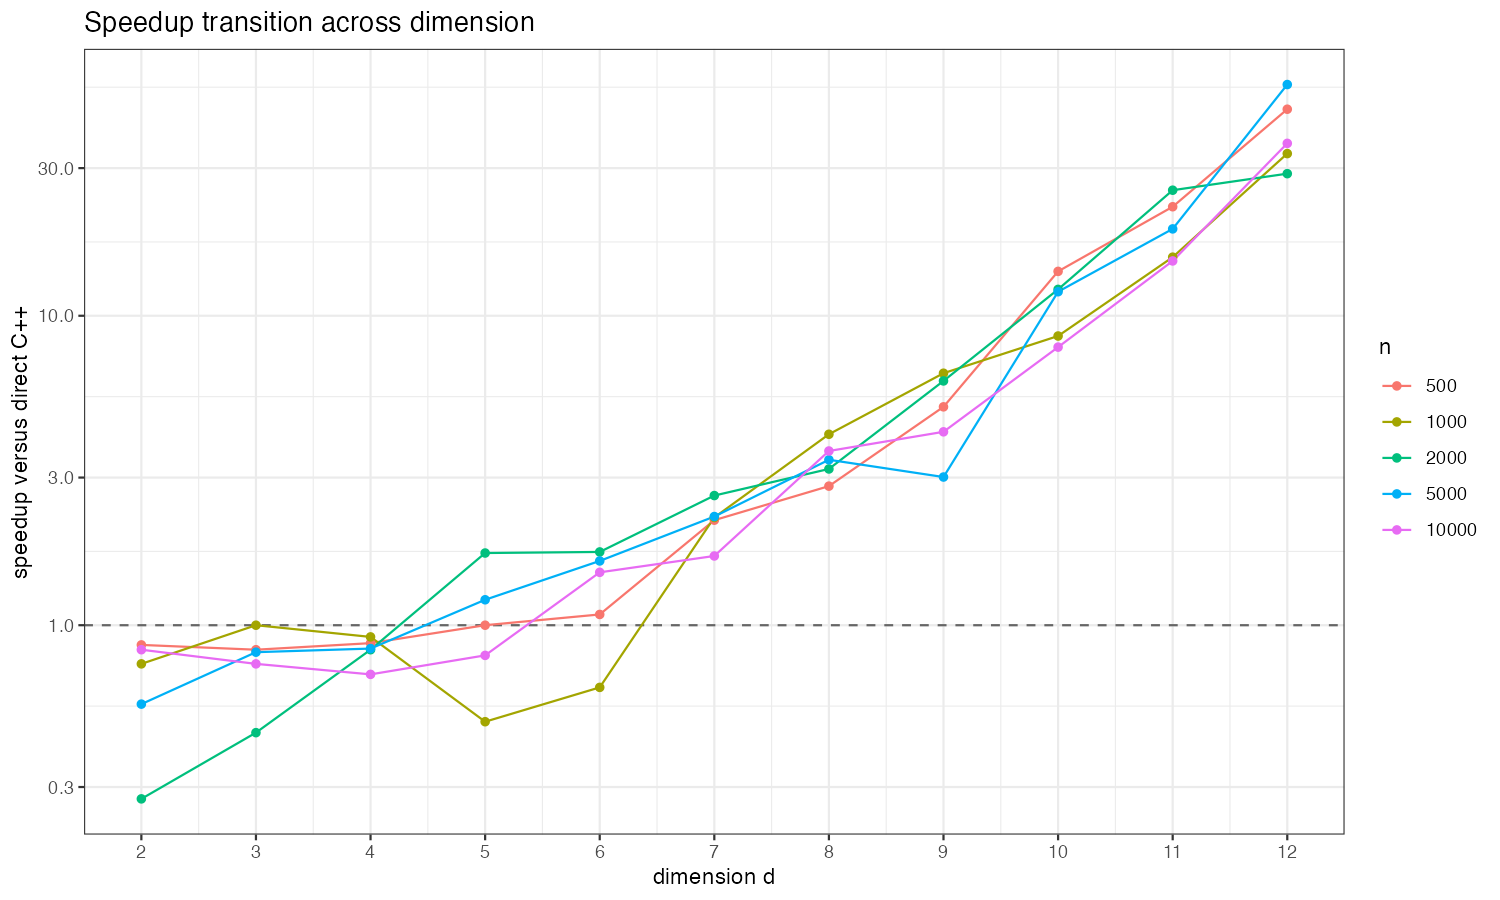
\includegraphics[width=0.95\textwidth]{../code/figures/scaling_speedup_by_dimension.png}
\caption{Median sparse-prefix speedup as a function of dimension for each tested sample size.}
\label{fig:scaling-lines}
\end{figure}

\begin{figure}[!htbp]
\centering
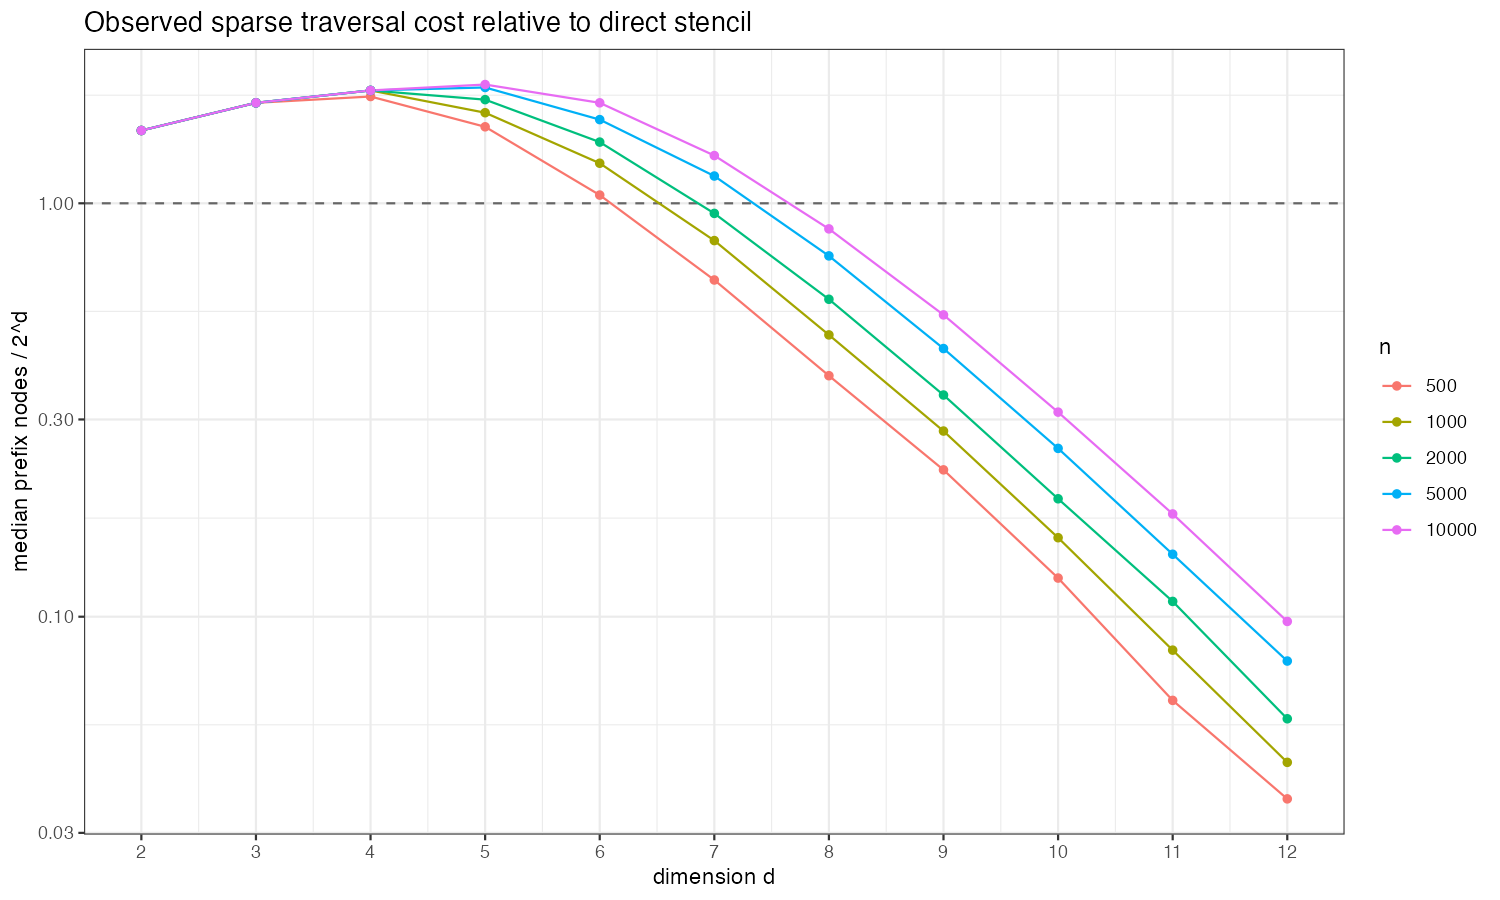
\includegraphics[width=0.95\textwidth]{../code/figures/scaling_prefix_ratio_by_dimension.png}
\caption{Median prefix-node ratio, defined as the number of tested prefix nodes divided by the nominal LBFP stencil size \(2^d\).}
\label{fig:scaling-prefix}
\end{figure}

\FloatBarrier

Together, Table~\ref{tab:scaling-transition} and Figures~\ref{fig:scaling-heatmap}--\ref{fig:scaling-prefix} support the cost-based interpretation in Proposition~\ref{prop:cost-criterion}: sparse-prefix traversal becomes favorable when the reduction in tested prefix nodes offsets the one-time index-construction cost.

\subsection{Occupancy-controlled validation of the cost criterion}

The scaling experiment above varies \(d\) and \(n\) through a data-generating mechanism. To isolate the role of grid occupancy, an occupancy-controlled LBFP benchmark was also run on artificial finite grids. The tested dimensions were \(d\in\{4,6,8,10,12\}\), with grid side lengths \(10,6,4,3,3\), respectively. These side lengths keep the artificial grid finite while allowing target occupancy fractions \(\rho\in\{0.001,0.005,0.01,0.05,0.10\}\). For each dimension and occupancy level, occupied cells were generated under two patterns: uniform occupancy and clustered occupancy. The estimator was evaluated at \(M=1000\) query points under two regimes: observation-like queries near occupied cells and random-grid queries over the finite grid.

For each configuration, the benchmark records \(G_{\mathrm{occ}}\), \(\bar p\), direct C++ time, sparse-prefix C++ time, and the cost ratio
\[
R_{\mathrm{cost}}
=
\frac{dG_{\mathrm{occ}}+M\bar p}{M|\stencil|}.
\]
The sparse-prefix mode is predicted when \(R_{\mathrm{cost}}<1\). Across the 100 configurations, this criterion selected the faster mode in 97 cases. The three mismatches occurred near the decision boundary, with sparse-prefix speedups between \(0.91\) and \(0.92\). The maximum absolute discrepancy between direct and sparse-prefix density values was \(1.39\times 10^{-17}\).

Table~\ref{tab:occupancy-criterion} summarizes the benchmark by dimension. The median speedup increases sharply from \(d=4\) to \(d=10\), while the median cost ratio decreases. This pattern is consistent with Proposition~\ref{prop:cost-criterion}: sparse-prefix traversal becomes favorable when the number of tested prefix nodes is small enough to compensate for the prefix-index construction term.

\begin{table}[!htbp]
\centering
\caption{Occupancy-controlled validation of the cost criterion. Each row summarizes 20 configurations, combining five target occupancies, two occupancy patterns, and two query regimes.}
\label{tab:occupancy-criterion}
\begin{tabular}{rrrr}
\toprule
\(d\) & median speedup & median \(R_{\mathrm{cost}}\) & criterion accuracy \\
\midrule
4  & 1.20 & 0.853 & 1.00 \\
6  & 1.66 & 0.566 & 0.95 \\
8  & 3.61 & 0.286 & 0.90 \\
10 & 11.70 & 0.121 & 1.00 \\
12 & 10.42 & 0.085 & 1.00 \\
\bottomrule
\end{tabular}
\end{table}

\begin{figure}[!htbp]
\centering
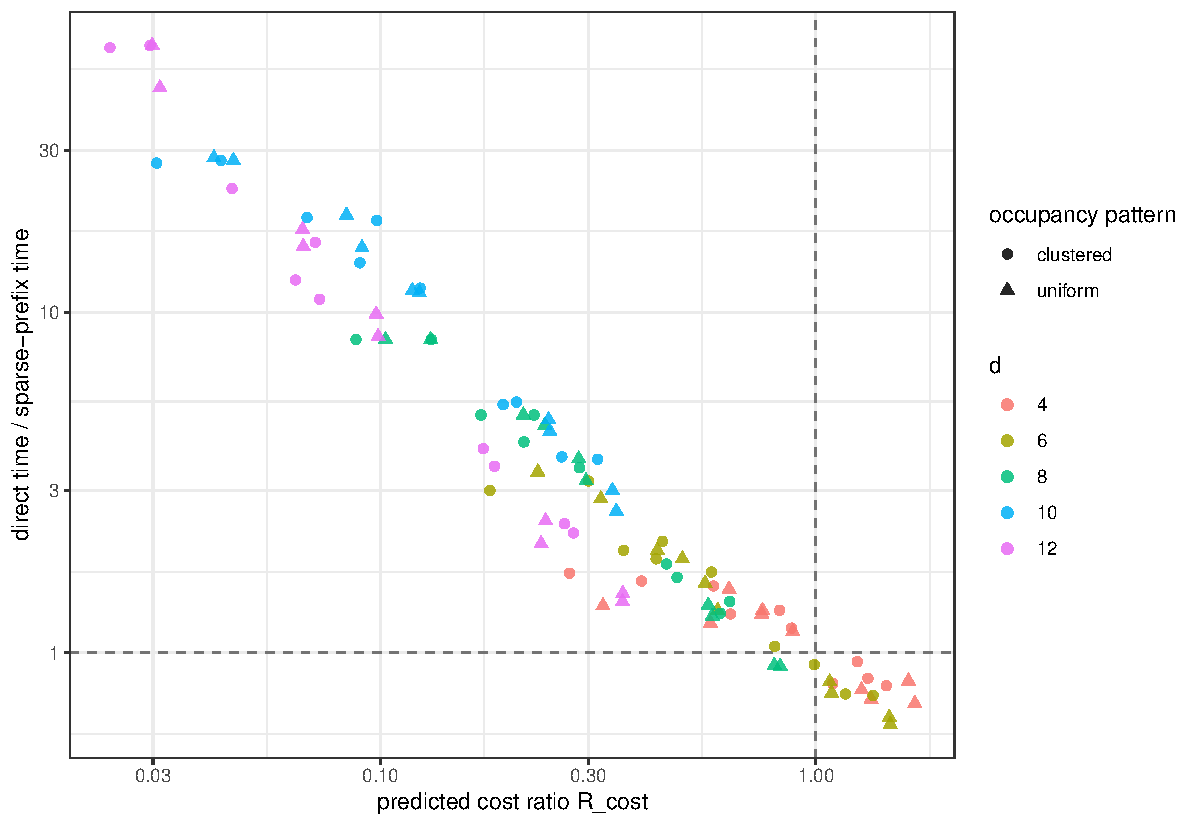
\includegraphics[width=0.9\textwidth]{../code/figures/cost_ratio_vs_speedup.pdf}
\caption{Observed sparse-prefix speedup versus the predicted cost ratio \(R_{\mathrm{cost}}\) in the occupancy-controlled benchmark. The vertical and horizontal reference lines mark the direct-versus-sparse transition.}
\label{fig:cost-ratio-speedup}
\end{figure}

\FloatBarrier

Together, Table~\ref{tab:occupancy-criterion} and Figure~\ref{fig:cost-ratio-speedup} show that the cost ratio tracks the observed direct-versus-sparse transition, with the remaining disagreements concentrated near the boundary.

\FloatBarrier

\subsection{Automatic mode selection}

The cost criterion can be used as a pilot-based automatic selector. For each occupancy-controlled configuration, a pilot subset of 100 query points was used to estimate \(\widehat{\bar p}\). Sparse-prefix evaluation was selected when
\[
dG_{\mathrm{occ}}+M\widehat{\bar p}
<
\tau M|\stencil|,
\qquad \tau=0.8.
\]
Both direct and sparse-prefix evaluation were then timed on the full query set, so the selected mode could be compared with the observed fastest mode. The selector chose the fastest mode in 93 of the 100 configurations. The median regret, defined as selected time divided by oracle time, was 1.00. The largest observed regret was 2.09, occurring in a high-occupancy random-grid configuration at \(d=8\). Errors relative to direct evaluation again remained at roundoff level, with maximum absolute error \(1.39\times 10^{-17}\).

Table~\ref{tab:mode-selector} reports selector performance by dimension. The selector is exact in all tested configurations for \(d=10\) and \(d=12\). Most errors occur at \(d=4\), where direct and sparse-prefix timings are close and the direct stencil has only 16 vertices. Thus the pilot rule is most reliable in the dimensions where the computational distinction is largest, and its main failure regime is the transition region where the two modes have similar cost.

\begin{table}[!htbp]
\centering
\caption{Automatic mode-selector performance with pilot size 100 and \(\tau=0.8\). Each row summarizes 20 configurations.}
\label{tab:mode-selector}
\begin{tabular}{rrrr}
\toprule
\(d\) & selector accuracy & median regret & maximum regret \\
\midrule
4  & 0.75 & 1.00 & 1.38 \\
6  & 0.95 & 1.00 & 1.00 \\
8  & 0.95 & 1.00 & 2.09 \\
10 & 1.00 & 1.00 & 1.00 \\
12 & 1.00 & 1.00 & 1.00 \\
\bottomrule
\end{tabular}
\end{table}

\begin{figure}[!htbp]
\centering
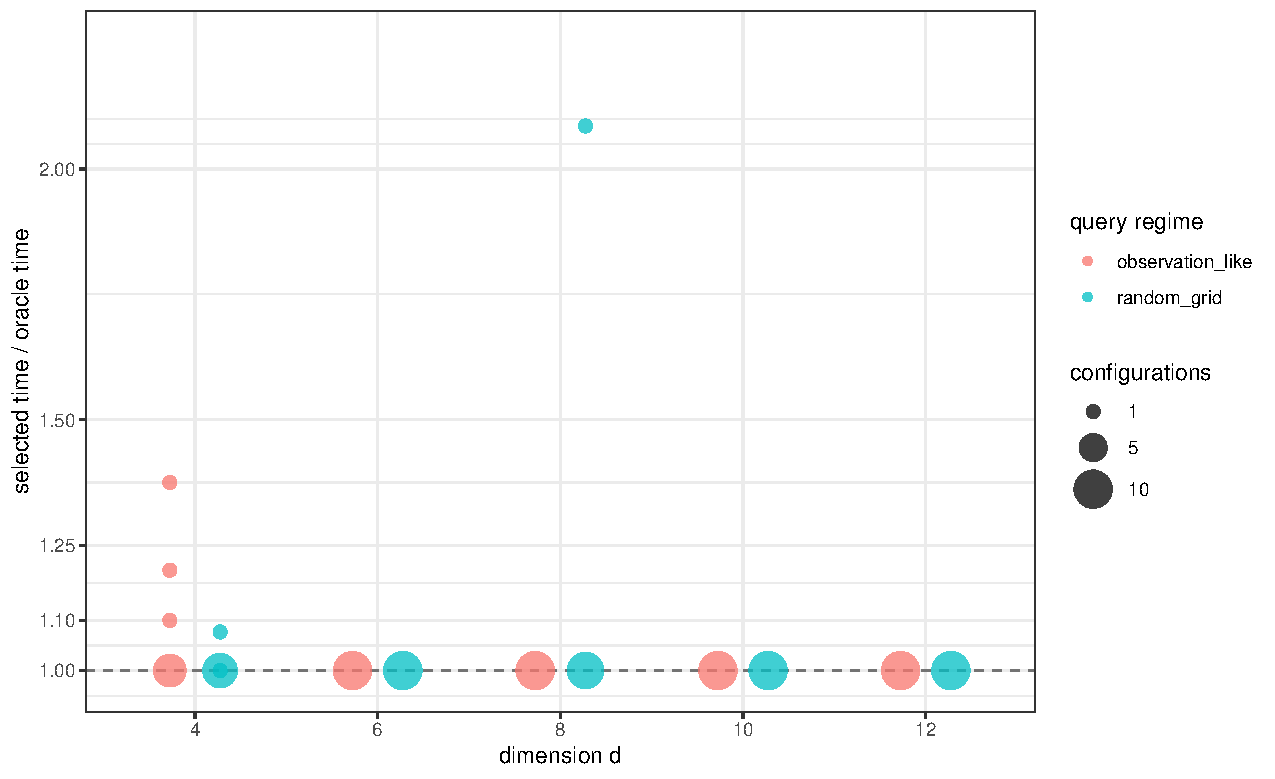
\includegraphics[width=0.95\textwidth]{../code/figures/mode_selector_regret.pdf}
\caption{Regret of the pilot-based automatic mode selector across the occupancy-controlled configurations. Point size indicates the number of configurations with the same plotted value. A regret of one indicates that the selected mode matched the oracle fastest mode.}
\label{fig:mode-selector-regret}
\end{figure}

\FloatBarrier

Together, Table~\ref{tab:mode-selector} and Figure~\ref{fig:mode-selector-regret} show that the selector has little or no regret in most tested configurations, with the largest regret occurring in the transition region.

\FloatBarrier

\section{Discussion}
\label{sec:discussion}

This section clarifies the scope of the method and the regimes in which sparse-prefix traversal is most relevant.

\subsection{Relation to sparse and convolutional computation}

The proposed method is best understood as an exact evaluation strategy for pointwise or observation-only finite-stencil density computations. In pointwise evaluation, \(M\) may be small, so the prefix-index construction cost must be amortized carefully. In observation-only evaluation, \(M=n\), as in leave-one-out or observation-level scoring, and Proposition~\ref{prop:cost-criterion} compares \(dG_{\mathrm{occ}}+M\bar p\) with \(M|\stencil|\). Sparse-prefix traversal is most relevant when the stencil is large and occupied grid cells represent a small fraction of the candidate local stencil branches.

This scope is different from full-grid convolutional smoothing. Binned KDEs with compactly supported kernels or explicitly truncated Gaussian kernels can be represented by finite local stencils. In contrast, untruncated Gaussian binned KDEs are more naturally treated as convolutional grid smoothers, especially when the full grid is evaluated. In that regime, separable convolution and FFT-based methods remain important alternatives \citep{Silverman1982FFT,Wand1994FastKDE,GramackiGramacki2017}. Sparse-prefix traversal is therefore not intended to replace full-grid convolution or FFT methods when the evaluation task, grid size, and smoothing structure favor those computations.

Sparse-prefix traversal is also not intended to replace optimized sparse tensor libraries. Tries, sorted coordinate fibers, compressed coordinate structures, or specialized sparse tensor kernels could reduce implementation constants \citep{Fredkin1960Trie,BaderKolda2007SparseTensor,KoldaBader2009TensorReview}. Such choices affect runtime, but they do not change the mathematical estimator, the exactness argument, or the cost criterion. The key statistical-computational point is that local grid-count estimators create many zero-count stencil candidates in sparse moderate-dimensional grids, and these candidates can be pruned exactly.

The broader computational choice depends on the estimator, grid occupancy, stencil size, prefix ordering, and evaluation task. Pointwise evaluation, observation-only evaluation, and full-grid surface estimation can favor different computational modes. The present experiments focus on exactness and on the direct-versus-sparse transition for finite-stencil evaluation; comparisons with optimized convolutional and sparse-tensor implementations are natural extensions for full-grid settings.

\section{Conclusion}

Local finite-stencil grid-count density estimators share a common computational form: each density value is a weighted sum over a finite stencil of grid counts. This article formulated histograms, LBFP, ASH, and GLBFP in that common form and studied exact sparse-prefix traversal as an alternative to direct stencil enumeration. The traversal prunes only zero-count branches, so the estimator is unchanged. The criterion \(dG_{\mathrm{occ}}+M\bar p<M|\stencil|\) gives a practical basis for choosing between direct and sparse evaluation and motivates a pilot-based mode selector. Numerical checks verified equality with direct evaluation at roundoff level, and the benchmarks identified sparse moderate-dimensional regimes where prefix pruning reduces computation. The framework therefore separates the statistical estimator from the computational mode, while making clear that the best mode depends on the stencil, occupancy, dimension, and evaluation task.

\section*{Declarations}

\paragraph{Funding}
The author received no specific funding for this work.

\paragraph{Competing interests}
The author declares that he has no known competing financial interests or personal relationships that could have appeared to influence the work reported in this paper.

\paragraph{Data availability}
The examples use synthetic data generated by the accompanying scripts. No external data are required to reproduce the numerical experiments.

\paragraph{Code availability}
The code, benchmark scripts, generated CSV outputs, figures, and session information are available in the public repository \url{https://github.com/AurelienNicosiaULaval/grid-density-sparse-traversal}.

\bibliography{references}

\end{document}
